%; whizzy document
% latex beamer presentation.
% platex, latex-beamer でコンパイルすることを想定。 

%     Tokyo Debian Meeting resources
%     Copyright (C) 2007 Junichi Uekawa
%     Copyright (C) 2007 Nobuhiro Iwamatsu   

%     This program is free software; you can redistribute it and/or modify
%     it under the terms of the GNU General Public License as published by
%     the Free Software Foundation; either version 2 of the License, or
%     (at your option) any later version.

%     This program is distributed in the hope that it will be useful,
%     but WITHOUT ANY WARRANTY; without even the implied warranty of
%     MERCHANTABILITY or FITNESS FOR A PARTICULAR PURPOSE.  See the
%     GNU General Public License for more details.

%     You should have received a copy of the GNU General Public License
%     along with this program; if not, write to the Free Software
%     Foundation, Inc., 51 Franklin St, Fifth Floor, Boston, MA  02110-1301 USA

% 実行順番
% sudo  ~/bin/usb-macbook-ir.c &
% real presentation (shell-command (concat "DISPLAY=:0.1 xpdf -fullscreen " (replace-regexp-in-string "tex$" "pdf"(buffer-file-name)) "&"))
% DISPLAY=:0.1 xpdf -fullscreen 

\documentclass[cjk,dvipdfmx,12pt]{beamer}
\usetheme{Tokyo}

%  preview (shell-command (concat "xpdf " (replace-regexp-in-string "tex$" "pdf"(buffer-file-name)) "&"))
%  presentation (shell-command (concat "xpdf -fullscreen " (replace-regexp-in-string "tex$" "pdf"(buffer-file-name)) "&"))

%http://www.naney.org/diki/dk/hyperref.html
%日本語EUC系環境の時
\AtBeginDvi{\special{pdf:tounicode EUC-UCS2}}
%シフトJIS系環境の時
%\AtBeginDvi{\special{pdf:tounicode 90ms-RKSJ-UCS2}}

\title{Debian on SuperH}
\subtitle{Debconf7}
\author{Nobuhiro Iwamatsu iwamatsu@debian.or.jp\\IRC nick: iwamatsu}
\date{Debconf7 06/17/2007}
\logo{
\includegraphics[width=8cm]{image200607/openlogo-light.eps}}



\begin{document}
\frame{\titlepage{}}

\section{What am I?}

\begin{frame}
 \frametitle{What am I?}
 \begin{itemize}
  \item Nobuhiro Iwamatsu
  \item Live in Japan ,Tokyo
  \item SuperH Linux Kernel Developer
  \item SH-IPL+g (SH bootloader) Maintainer and u-boot SH Maintainer
  \item In New Maintainer process
    
 \end{itemize}
\end{frame}


\section{What is SuperH?}

\begin{frame}
 \frametitle{What is SuperH?}
 \begin{itemize}
  \item Made by Renesas Technology Corp.
  \item Embedded CPU used well in Japan and Europe.
  \item Many kinds of CPU.
  
	SH1/SH2/SH2A/SH3/SH3-DSP/SH4/SH4A/SH4A-DSP/SH64 .....

  \item Used for NAS, cellular phone, LCD TV controller , and etc...
  \item Linux is working .
    
 \end{itemize}
\end{frame}

\section{History}

\begin{frame}
 \frametitle{History}
 
\end{frame}

\begin{frame}
 \frametitle{The 1st SuperH porting}
  \begin{itemize}
    \item Began to port Linux in Japan in 1999 .
    \item Began port to Debian with Mr.Yaegashi Mr.Ishikawa Mr.Bolzer in 2000.
    \item Support targets are SH3/SH4 .
    \item Development stop in 2003. 
  \end{itemize}
\end{frame}

\begin{frame}
 \frametitle{The 2nd SuperH porting}
  \begin{itemize}
    \item LANDISK and LANTANK\footnote{Lantank and landisk are NAS} were sold from the I/O-DATA in 2003 and 2005.
    \item Use Linux and Debian :-) . Ported by I/O HACK porject users.
    \item The book and the feature of a lot of LANDISK/LANTANK were united. 
    \item Packages were old.
    \item Renesas can not inability to follow this project.
  \end{itemize}
\end{frame}


\begin{frame}
 \frametitle{LANDISK/LANTANK}

\begin{figure}
 \begin{minipage}[t]{0.6\hsize}
   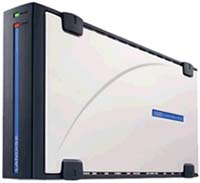
\includegraphics[width=0.5\hsize]{image200705/landisk00.jpg}
 \end{minipage}
 \begin{minipage}[t]{0.5\hsize}
  \begin{itemize}
   \item SH7751R( 266Mhz )
   \item 64MB RAM
   \item UDMA133 PATA 
   \item 10/100Base-T x1
   \item USB2.0 x2 
  \end{itemize}
 \end{minipage}
\end{figure}
\end{frame}

\begin{frame}
 \frametitle{Doesn't repeat the history.....}

  I began porting to SH of Debian in August 2006 .\\
  Because ...
  \begin{itemize}
    \item I 'm Debian user and in NM process.
    \item I want the distribution to which SH is supported.

	Gentoo? I don't want to use that.
    %\item I want to use Debian on business. :-)
    \item I want to enable the user of SH to use Debian.
  \end{itemize}
\end{frame}



\begin{frame}
 \frametitle{Influence}
    \begin{itemize}
	\item Aspect from Debian Project
	 \begin{itemize}
	  \item Debian users of Embedded number up.
	  \item We can approach the conquest of the 
		correspondence architecture.%by one step. 
 
	 \end{itemize} 
	\item Aspect from SuperH User/Developer
	 \begin{itemize}
	  \item They becomes easy to develop SuperH. 
	 \end{itemize}
  \end{itemize}
\end{frame}


%\begin{frame}
% \frametitle{ポーティングされることによって、いいことは?}
%\begin{itemize}
%  \item Debian からみたいいところ
%	Debian users of Embedded increases. 
%	
%	世界制服へ一歩近づく%
%
%
%  \item SH 側からみた場合のいいところ
%  	SH user can use.
%  	製品化が敷居が下がる。現状では、テストする環境を自分だけでつくっている。
%  	ホビーユーザーは使い易くなる。いまはマトモに使えるディストリがない。
%	サポートしたディストリができる。
%	ワークフローとか。 
%\end{itemize}
%\end{frame}

\section{My Plan}
\begin{frame}
 \frametitle{My Plan}
 \begin{itemize}
  \item Support architecture in Debian
    
	SH4 only. 
	I plan to support the little endian first .

  \item Don't build SH3 binary packages

	However, there is the following problems. 
	\begin{itemize}
	  \item about FPU
	  \item about calling convention issue
	  \item about Cache issue
	\end{itemize}

	When these are solved , it is possible to 
	work in SH3 by the SH4 binary. 
	
%	A big difference between SH3 and SH4 is 
%	whether it is or doesn't exist about FPU.
%	Because the FPU emulation was supported with linux-kernel.
%	The binary of SH4 can be moved on the SH3 machine. 
%	I plan to support this method.  
	

  \item Big endian support

	I plan to support the big endian after little endian.
  
 \end{itemize}
\end{frame}

\section{Now states}

\begin{frame}
 \frametitle{Now states}
 \begin{itemize}
  \item Discussion in Mailing list.
  \item SH4 Support only.
  \item Build-essential's packages is built.
  \item Local buildd working.
  \item SH4 debootstrap is working.
  \item Some package built (about 2000 packages)
 \end{itemize}
\end{frame}

\begin{frame}
 \frametitle{Development Machine}
\end{frame}

\begin{frame}
 \frametitle{LANTANK x 3}
  \begin{center}
  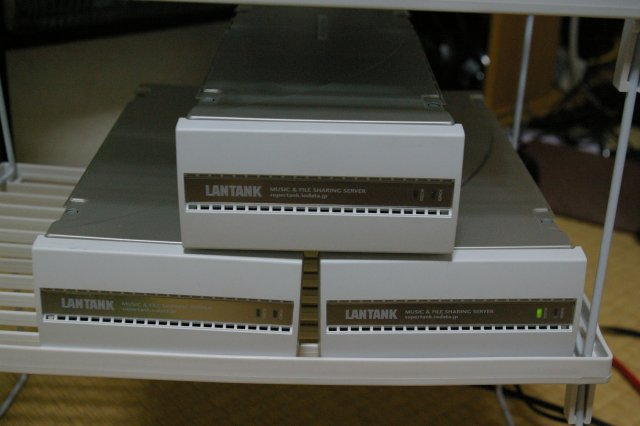
\includegraphics[width=0.7\hsize]{image200705/lantank01.jpg}
  \end{center}
\end{frame}

\begin{frame}
 \frametitle{RTS7751R2D}
 \begin{minipage}[t]{0.4\hsize}
  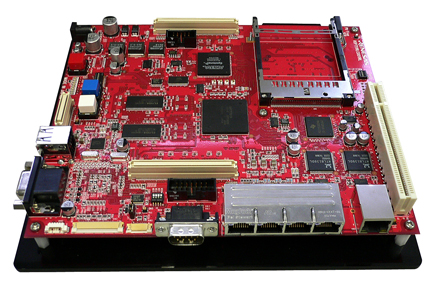
\includegraphics[width=1.0\hsize]{image200705/r2d.jpg}
 \end{minipage} 
 \begin{minipage}[t]{0.5\hsize}
  \begin{itemize}
   \item SH7751R ( 266Mhz )
   \item 64MB RAM
   \item 4MB Flash 
   \item CF slot 
   \item 1 100base Ethernet
   \item PCI Bus 
  \end{itemize}
 \end{minipage}
\end{frame}

\begin{frame}
 \frametitle{Developer}
  %This project has gone basically only by me.
  Only I and dancerj , now.
 
\end{frame}

\begin{frame}
 \frametitle{Support member}
  However, I have the people who help development. 
 \begin{itemize}
  \item kmuto

	Debian Developer \\
	Support build buildd.

  \item kkojima

	GNU binutils SH maintainer \\
	Support SH specific.

  \item kinneko

	I/O Hack member\\
	He is tested SH's debian packages.	

  \item gotom
 
 	Debian Developer

	I presented SH development board for him. But he doesn't work.

%  \item dancerj
%
%	Debian Developer
	
	
 \end{itemize}
\end{frame}


\begin{frame}
 \frametitle{Need developper}
 I am looking for the person who develops together :-)

\end{frame}


\section{Todo}
\begin{frame}
 \frametitle{Todo}

   \begin{itemize}
    %\item build all sid package.
    \item To official support architecture.
    \item Registration to buildd.net.
    \item Create SH port and buildd maintainance team.
    \item Send SH specific patch to Package Maintainer.
    \item Keep buildd network.
   \end{itemize}
\end{frame}

\begin{frame}
 \frametitle{Get SH devices}
You will be able to participate in development with the following devices if you are interested in the development of Debian on SuperH. 

\end{frame}



\begin{frame}
 \frametitle{Get SH devices}
 \begin{minipage}[t]{0.3\hsize}
  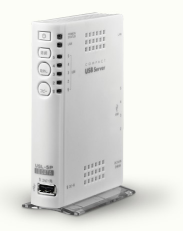
\includegraphics[width=1.0\hsize]{image200705/usl5p.png}
 \end{minipage} 
 \begin{minipage}[t]{0.3\hsize}
  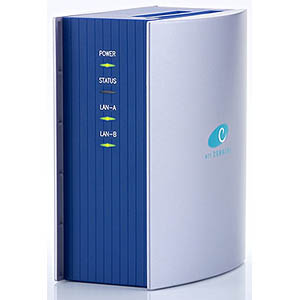
\includegraphics[width=1.0\hsize]{image200705/lbox.jpg}
 \end{minipage} 
 \begin{minipage}[t]{0.3\hsize}
  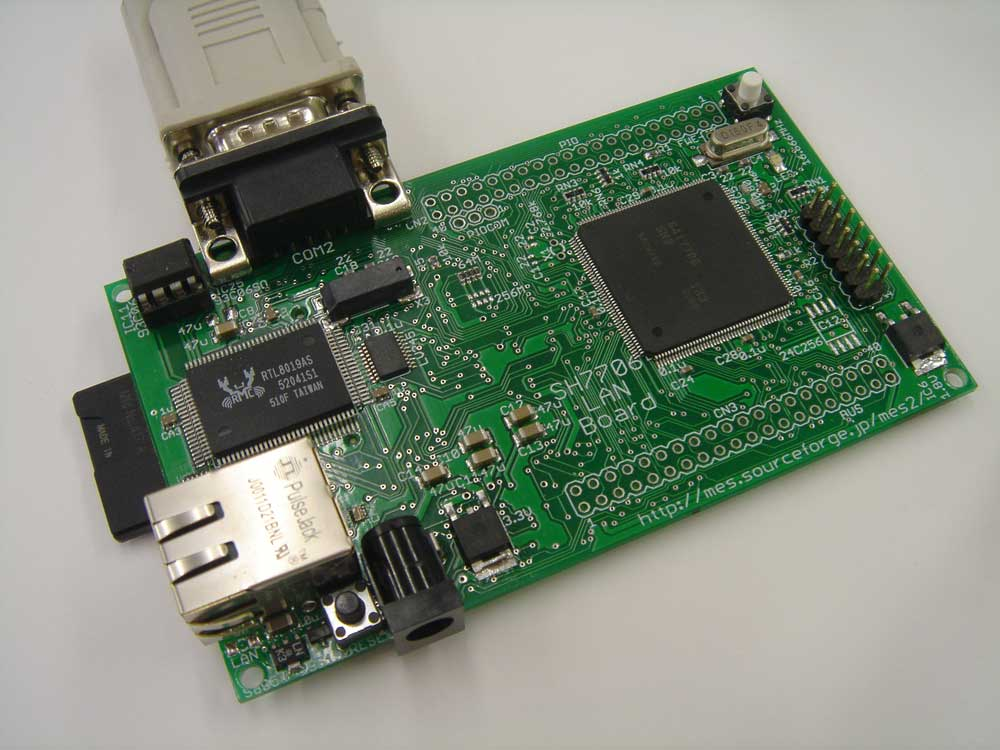
\includegraphics[width=1.0\hsize]{image200705/t-sh7706lan.jpg}
 \end{minipage} 
 \begin{minipage}[t]{0.4\hsize}
  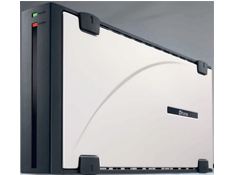
\includegraphics[width=1.0\hsize]{image200705/PX-EH16L.png}
 \end{minipage} 

\end{frame}


\begin{frame}
 \frametitle{USL-5P}
 \begin{minipage}[t]{0.4\hsize}
  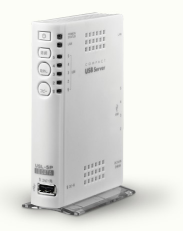
\includegraphics[width=0.8\hsize]{image200705/usl5p.png}
 \end{minipage} 
 \begin{minipage}[t]{0.5\hsize}
  \begin{itemize}
   \item SH7751R ( 266Mhz )
   \item 64MB RAM 
   \item CF slot 
   \item 1 100base Ethernet
   \item USB2.0 port x 5
   \item about \$100
  \end{itemize}
 \end{minipage}
\end{frame}

\begin{frame}
 \frametitle{L-BOX}
 \begin{minipage}[t]{0.4\hsize}
  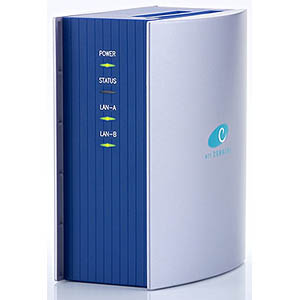
\includegraphics[width=1.0\hsize]{image200705/lbox.jpg}
 \end{minipage} 
 \begin{minipage}[t]{0.5\hsize}
  \begin{itemize}
   \item SH7751R ( 266Mhz )
   \item 64MB RAM 
   \item CF slot 
   \item 2 100base Ethernet
   \item 1 CardBus Slot
   \item about \$500 
  \end{itemize}
 \end{minipage}
\end{frame}

\begin{frame}
 \frametitle{T-SH7706-LAN}
 \begin{minipage}[t]{0.4\hsize}
  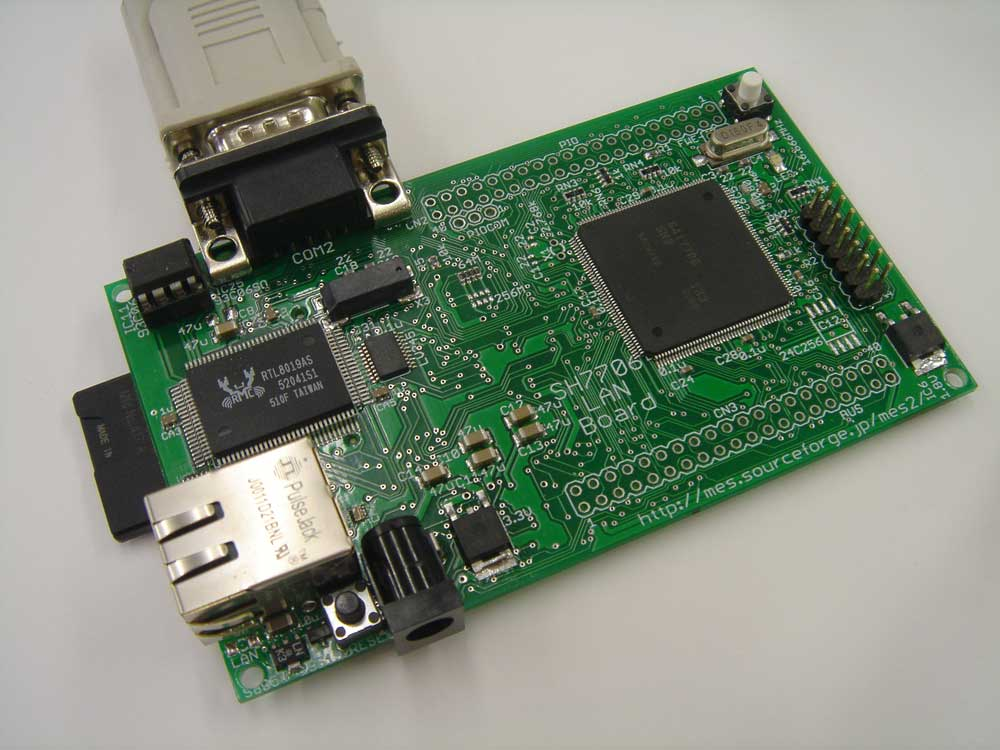
\includegraphics[width=1.0\hsize]{image200705/t-sh7706lan.jpg}
 \end{minipage} 
 \begin{minipage}[t]{0.5\hsize}
  \begin{itemize}
   \item SH7706 ( 133Mhz )
   \item 32MB RAM 
   \item MMC slot 
   \item 1 100base Ethernet
   \item about \$70
  \end{itemize}
 \end{minipage}
\end{frame}

\begin{frame}
 \frametitle{PX-EH16L}
 \begin{minipage}[t]{0.4\hsize}
  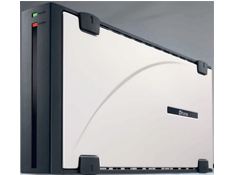
\includegraphics[width=1.0\hsize]{image200705/PX-EH16L.png}
 \end{minipage} 
 \begin{minipage}[t]{0.5\hsize}
  \begin{itemize}
   \item SH7751R( 266Mhz )
   \item 64BM RAM
   \item UDMA133 PATA 
   \item 10/100Base-T x1
   \item USB2.0 x2 
   \item about \$300 (This can be bought in Europe.)
  \end{itemize}
 \end{minipage}
\end{frame}


%\begin{frame}
% \frametitle{LANDISK Pro}
%  This is name looks like , but SH is not installed . Note analogous articles. 
%  \begin{center}
%  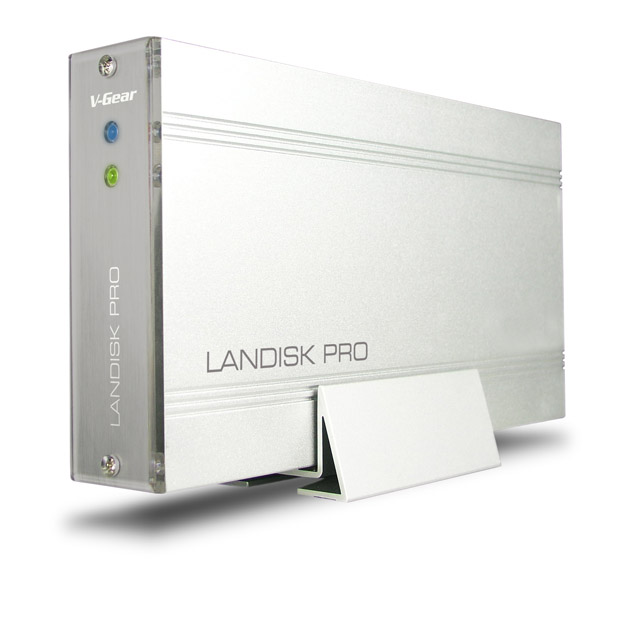
\includegraphics[width=0.7\hsize]{image200705/landisk_fake.jpg}
%  \end{center}
%\end{frame}


\begin{frame}

 \frametitle{Links}
   \begin{itemize}
    \item SuperH 
		
		\url{http://www.renesas.com}
    \item IRC 

		\#debian-superh @ oftc.net
    \item Mailing List

		debian-superh@debian.org
    \item Wiki 

		http://wiki.debian.org/SHPort
    \item Debian Packages repsitory

	\url{http://www.nigauri.org/~iwamatsu/debian/debian-sh4/}

  \item iohack

	\url{http://iohack.sourceforge.jp}
   \end{itemize}
\end{frame}

\section{Question}
\begin{frame}
 \frametitle{Any question?}

\end{frame}


\end{document}
